\documentclass{ximera}

 

\usepackage{epsfig}

\graphicspath{
  {./}
  {figures/}
}

\usepackage{morewrites}
\makeatletter
\newcommand\subfile[1]{%
\renewcommand{\input}[1]{}%
\begingroup\skip@preamble\otherinput{#1}\endgroup\par\vspace{\topsep}
\let\input\otherinput}
\makeatother

\newcommand{\includeexercises}{\directlua{dofile("/home/jim/linearAlgebra/laode/exercises.lua")}}

%\newcounter{ccounter}
%\setcounter{ccounter}{1}
%\newcommand{\Chapter}[1]{\setcounter{chapter}{\arabic{ccounter}}\chapter{#1}\addtocounter{ccounter}{1}}

%\newcommand{\section}[1]{\section{#1}\setcounter{thm}{0}\setcounter{equation}{0}}

%\renewcommand{\theequation}{\arabic{chapter}.\arabic{section}.\arabic{equation}}
%\renewcommand{\thefigure}{\arabic{chapter}.\arabic{figure}}
%\renewcommand{\thetable}{\arabic{chapter}.\arabic{table}}

%\newcommand{\Sec}[2]{\section{#1}\markright{\arabic{ccounter}.\arabic{section}.#2}\setcounter{equation}{0}\setcounter{thm}{0}\setcounter{figure}{0}}

\newcommand{\Sec}[2]{\section{#1}}

\setcounter{secnumdepth}{2}
%\setcounter{secnumdepth}{1} 

%\newcounter{THM}
%\renewcommand{\theTHM}{\arabic{chapter}.\arabic{section}}

\newcommand{\trademark}{{R\!\!\!\!\!\bigcirc}}
%\newtheorem{exercise}{}

\newcommand{\dfield}{{\sf dfield9}}
\newcommand{\pplane}{{\sf pplane9}}

\newcommand{\EXER}{\section*{Exercises}}%\vspace*{0.2in}\hrule\small\setcounter{exercise}{0}}
\newcommand{\CEXER}{}%\vspace{0.08in}\begin{center}Computer Exercises\end{center}}
\newcommand{\TEXER}{} %\vspace{0.08in}\begin{center}Hand Exercises\end{center}}
\newcommand{\AEXER}{} %\vspace{0.08in}\begin{center}Hand Exercises\end{center}}

% BADBAD: \newcommand{\Bbb}{\bf}

\newcommand{\R}{\mbox{$\Bbb{R}$}}
\newcommand{\C}{\mbox{$\Bbb{C}$}}
\newcommand{\Z}{\mbox{$\Bbb{Z}$}}
\newcommand{\N}{\mbox{$\Bbb{N}$}}
\newcommand{\D}{\mbox{{\bf D}}}
\usepackage{amssymb}
%\newcommand{\qed}{\hfill\mbox{\raggedright$\square$} \vspace{1ex}}
%\newcommand{\proof}{\noindent {\bf Proof:} \hspace{0.1in}}

\newcommand{\setmin}{\;\mbox{--}\;}
\newcommand{\Matlab}{{M\small{AT\-LAB}} }
\newcommand{\Matlabp}{{M\small{AT\-LAB}}}
\newcommand{\computer}{\Matlab Instructions}
\newcommand{\half}{\mbox{$\frac{1}{2}$}}
\newcommand{\compose}{\raisebox{.15ex}{\mbox{{\scriptsize$\circ$}}}}
\newcommand{\AND}{\quad\mbox{and}\quad}
\newcommand{\vect}[2]{\left(\begin{array}{c} #1_1 \\ \vdots \\
 #1_{#2}\end{array}\right)}
\newcommand{\mattwo}[4]{\left(\begin{array}{rr} #1 & #2\\ #3
&#4\end{array}\right)}
\newcommand{\mattwoc}[4]{\left(\begin{array}{cc} #1 & #2\\ #3
&#4\end{array}\right)}
\newcommand{\vectwo}[2]{\left(\begin{array}{r} #1 \\ #2\end{array}\right)}
\newcommand{\vectwoc}[2]{\left(\begin{array}{c} #1 \\ #2\end{array}\right)}

\newcommand{\ignore}[1]{}


\newcommand{\inv}{^{-1}}
\newcommand{\CC}{{\cal C}}
\newcommand{\CCone}{\CC^1}
\newcommand{\Span}{{\rm span}}
\newcommand{\rank}{{\rm rank}}
\newcommand{\trace}{{\rm tr}}
\newcommand{\RE}{{\rm Re}}
\newcommand{\IM}{{\rm Im}}
\newcommand{\nulls}{{\rm null\;space}}

\newcommand{\dps}{\displaystyle}
\newcommand{\arraystart}{\renewcommand{\arraystretch}{1.8}}
\newcommand{\arrayfinish}{\renewcommand{\arraystretch}{1.2}}
\newcommand{\Start}[1]{\vspace{0.08in}\noindent {\bf Section~\ref{#1}}}
\newcommand{\exer}[1]{\noindent {\bf \ref{#1}}}
\newcommand{\ans}{}
\newcommand{\matthree}[9]{\left(\begin{array}{rrr} #1 & #2 & #3 \\ #4 & #5 & #6
\\ #7 & #8 & #9\end{array}\right)}
\newcommand{\cvectwo}[2]{\left(\begin{array}{c} #1 \\ #2\end{array}\right)}
\newcommand{\cmatthree}[9]{\left(\begin{array}{ccc} #1 & #2 & #3 \\ #4 & #5 &
#6 \\ #7 & #8 & #9\end{array}\right)}
\newcommand{\vecthree}[3]{\left(\begin{array}{r} #1 \\ #2 \\
#3\end{array}\right)}
\newcommand{\cvecthree}[3]{\left(\begin{array}{c} #1 \\ #2 \\
#3\end{array}\right)}
\newcommand{\cmattwo}[4]{\left(\begin{array}{cc} #1 & #2\\ #3
&#4\end{array}\right)}

\newcommand{\Matrix}[1]{\ensuremath{\left(\begin{array}{rrrrrrrrrrrrrrrrrr} #1 \end{array}\right)}}

\newcommand{\Matrixc}[1]{\ensuremath{\left(\begin{array}{cccccccccccc} #1 \end{array}\right)}}



\renewcommand{\labelenumi}{\theenumi)}
\newenvironment{enumeratea}%
{\begingroup
 \renewcommand{\theenumi}{\alph{enumi}}
 \renewcommand{\labelenumi}{(\theenumi)}
 \begin{enumerate}}
 {\end{enumerate}\endgroup}



\newcounter{help}
\renewcommand{\thehelp}{\thesection.\arabic{equation}}

%\newenvironment{equation*}%
%{\renewcommand\endequation{\eqno (\theequation)* $$}%
%   \begin{equation}}%
%   {\end{equation}\renewcommand\endequation{\eqno \@eqnnum
%$$\global\@ignoretrue}}

%\input{psfig.tex}

\author{Martin Golubitsky and Michael Dellnitz}

%\newenvironment{matlabEquation}%
%{\renewcommand\endequation{\eqno (\theequation*) $$}%
%   \begin{equation}}%
%   {\end{equation}\renewcommand\endequation{\eqno \@eqnnum
% $$\global\@ignoretrue}}

\newcommand{\soln}{\textbf{Solution:} }
\newcommand{\exercap}[1]{\centerline{Figure~\ref{#1}}}
\newcommand{\exercaptwo}[1]{\centerline{Figure~\ref{#1}a\hspace{2.1in}
Figure~\ref{#1}b}}
\newcommand{\exercapthree}[1]{\centerline{Figure~\ref{#1}a\hspace{1.2in}
Figure~\ref{#1}b\hspace{1.2in}Figure~\ref{#1}c}}
\newcommand{\para}{\hspace{0.4in}}

\renewenvironment{solution}{\suppress}{\endsuppress}

\ifxake
\newenvironment{matlabEquation}{\begin{equation}}{\end{equation}}
\else
\newenvironment{matlabEquation}%
{\let\oldtheequation\theequation\renewcommand{\theequation}{\oldtheequation*}\begin{equation}}%
  {\end{equation}\let\theequation\oldtheequation}
\fi

\makeatother


\title{Uncoupled Linear Systems of Two Equations}

\begin{document}
\begin{abstract}
\end{abstract}
\maketitle


\label{sec:UncoupledLS}

A system of two linear ordinary differential equations \index{system of differential equations}
has the form
\renewcommand{\arraystretch}{1.8}
\begin{equation} \label{e:autlin}
\begin{array}{lll}
\dps \frac{dx}{dt}(t)  & = & a x(t) + b y(t) \\
\dps \frac{dy}{dt}(t)  & = & c x(t) + d y(t),
\end{array}
\end{equation}
\renewcommand{\arraystretch}{1.0}%
where $a,b,c,d$ are real constants.  Solutions of \eqref{e:autlin} are 
pairs of functions $(x(t),y(t))$.  

A solution to the planar system \eqref{e:autlin} that is constant in time $t$ is called 
an {\em equilibrium}.  Observe that the origin $(x(t),y(t))=(0,0)$ is always an equilibrium 
solution to the linear system \eqref{e:autlin}. 

We begin our discussion of linear systems of 
differential equations by considering uncoupled
\index{system of differential equations!uncoupled}systems of the form
\renewcommand{\arraystretch}{1.8}
\begin{equation} \label{lin2}
\begin{array}{lll}
\dps \frac{dx}{dt}(t) & = & a x(t) \\
\dps \frac{dy}{dt}(t) & = & d y(t).
\end{array}
\end{equation}
\renewcommand{\arraystretch}{1.0}%
Since the system is {\em uncoupled\/} (that is, the equation for
$\dot{x}$ does not depend on $y$ and the equation for $\dot{y}$
does not depend on $x$), we can solve this system by solving each
equation independently, as we did for \eqref{lin1}:
\begin{equation} \label{e:explicitsoln}
\begin{array}{ccc}
x(t) & = & x_0e^{at} \\
y(t) & = & y_0e^{dt}.
\end{array}
\end{equation}
There are now two initial conditions that are identified by
\[
x(0) = x_0 \AND y(0) = y_0.
\]

Having found all the solutions to \eqref{lin2} in \eqref{e:explicitsoln},
we now explore the geometry of the phase plane for
these uncoupled systems both analytically and by using \Matlabp.


\subsection*{Asymptotic Stability of the Origin}

As we did for the single equation \eqref{lin1}, we ask
what happens to solutions to \eqref{lin2} starting at $(x_0,y_0)$ as
time $t$ increases.  That is, we compute
\[
\lim_{t\to\infty}(x(t),y(t))=\lim_{t\to\infty}(x_0e^{a t},y_0e^{d t}).
\]
This limit is $(0,0)$ when both $a<0$ and $d<0$; but
if either $a$ or $d$ is positive, then most solutions diverge
to infinity, since either
\[
\lim_{t\to\infty}|x(t)| =\infty \quad \mbox{ or } \quad
\lim_{t\to\infty}|y(t)| =\infty.
\]


Roughly speaking, an equilibrium \index{equilibrium} $(x_0,y_0)$ is 
{\em asymptotically stable\/} \index{stability!asymptotic} if every 
trajectory $(x(t),y(t))$ beginning from an initial condition near 
$(x_0,y_0)$ stays near $(x_0,y_0)$ for all positive $t$, and
\[
\lim_{t\to\infty}(x(t),y(t)) = (x_0,y_0).
\]
The equilibrium is {\em unstable\/} \index{unstable} if there are  
trajectories with initial conditions arbitrarily close to the 
equilibrium that move far away from that equilibrium.

At this stage, it is not clear how to determine whether the
origin is asymptotically stable for a general linear system
\eqref{e:autlin}.  However, for uncoupled linear systems we
have shown that the origin is an asymptotically stable
equilibrium when both $a < 0$ and $d < 0$.  If either
$a >0$ or $d > 0$, then $(0,0)$ is unstable.

\subsubsection*{Invariance of the Axes}

There is another observation that we can make
for uncoupled systems.  Suppose that the initial condition for
an uncoupled system lies on the $x$-axis; that is, suppose $y_0=0$.
Then the solution $(x(t),y(t))=(x_0e^{at},0)$ also lies on the
$x$-axis for all time.  Similarly, if the initial condition lies
on the $y$-axis, then the solution $(0,y_0e^{dt})$ lies on the
$y$-axis for all time.

This invariance of the coordinate axes for uncoupled systems
follows directly from \eqref{e:explicitsoln}.  It turns out that
many linear systems of differential equations have invariant
lines; this is a topic to which we return later in this chapter.

\subsection*{Generating Phase Space Pictures with {\pplane}}
\index{\computer!pplane8}

How can we visualize a solution $(x(t),y(t))$ in \eqref{e:explicitsoln} 
to the system of differential equations \eqref{lin2}?  The time series approach
suggests that we should graph $(x(t),y(t))$ as a function of $t$;
that is, we should plot the curve
\[
(t,x(t),y(t))
\]
in three dimensions.  Using \Matlab it is
possible to plot such a graph --- but such a graph by itself is
difficult to interpret.  Alternatively, we could graph either of
the functions $x(t)$ or $y(t)$ by themselves as we do for
solutions to single equations --- but then some information is
lost.

The method we prefer is the {\em phase space\/}\index{phase!space} 
plot obtained by thinking of $(x(t),y(t))$ as the
position of a particle in the $xy$-plane at time $t$.  We then
graph the point $(x(t),y(t))$ in the plane as $t$ varies.  When
looking at phase space plots, it is natural to call solutions
{\em trajectories\/},\index{trajectory} since we can imagine
that we are watching a particle moving in the plane as time
changes.

We begin by considering uncoupled linear equations.  As we saw,
when the initial conditions are on a coordinate axis (either
$(x_0,0)$ or $(0,y_0)$), the solutions remain on that coordinate
axis for all time $t$.  For these initial conditions, the equations behave as if
they were one dimensional.  However, if we consider an initial
condition $(x_0,y_0)$ that is not on a coordinate axis, then even
for an uncoupled system it is a little difficult to
{\em see\/} what the trajectory looks like.  At this point
it is useful to use the computer.

The method used to integrate planar systems of 
differential equations is similar to that used to integrate
single equations.  The solution
curve $(x(t),y(t))$ to \eqref{lin2} at a point $(x_0,y_0)$ is
tangent to the direction $(f,g) = (ax_0 + by_0, cx_0. + dy_0)$.  So
the differential equation solver plots the direction field
\index{direction field}
$(f,g)$ and then finds curves that are tangent to these
vectors at each point in time.

The program {\pplane}\index{\computer!pplane8}, written by John
Polking,\index{Polking, John} draws two-dimensional phase planes.  
In \Matlab type
\begin{verbatim}
pplane9
\end{verbatim}
and the window with the {\sf PPLANE9 Setup} appears. {\pplane}
has a number of preprogrammed differential equations listed in a
menu accessed by clicking on {\sf Gallery}.  To explore linear
systems, choose {\sf linear system} in the {\sf Gallery}.  (Note that the 
parameters in the {\sf linear system} are given by capitals rather than 
lower case {\sf a,b,c,d}.)

To integrate the uncoupled linear system, set the parameters $b$
and $c$ equal to zero. We now have the system \eqref{lin2} with
$a = 2$ and $d = -3$.  After pushing {\sf Proceed}, a display window
appears. In this window the plane is filled by vectors $(f,g)$ indicating 
directions.

We may start the computations by clicking
with a mouse button on an initial value $(x_0,y_0)$.  For example,
if we click approximately onto $(x(0),y(0))=(x_0,y_0)=(1,1)$, then
the trajectory in the upper right quadrant of
Figure~\ref{pp_dsp1} displays.

\begin{figure*}[htb]
     \centerline{%
     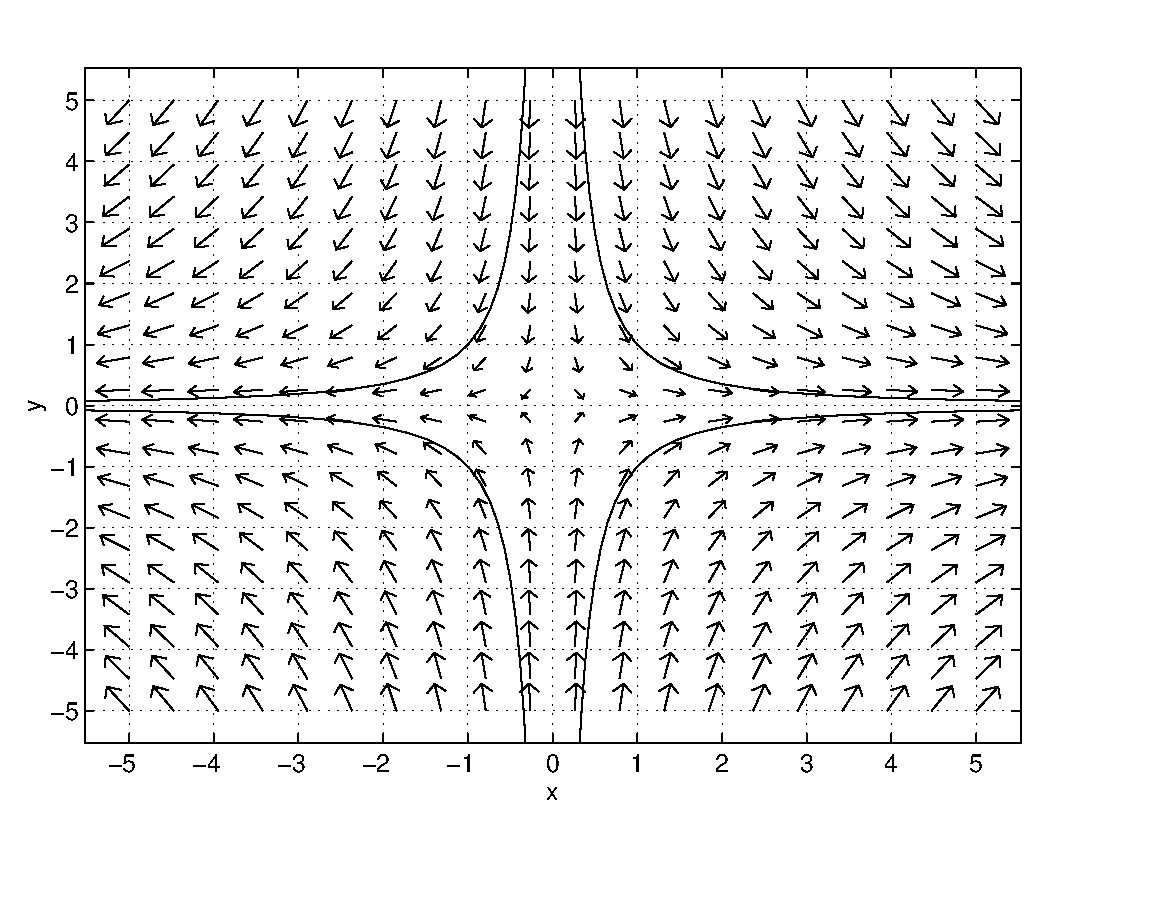
\psfig{file=../figures/pp_dsp1.eps,width=3.5in}}
     \caption{{\sf PPLANE9 Display} for \protect\eqref{lin2} with
             $a=2$, $d=-3$ and $x,y\in [-5,5]$. Solutions
             going through $(\pm 1,\pm 1)$ are shown.}
     \label{pp_dsp1}
\end{figure*}

First {\pplane} draws the trajectory in forward time for
$t\ge 0$ and then it draws the trajectory in backwards time for
$t\le 0$.  More precisely, when we click on a point $(x_0,y_0)$ in
the $(x,y)$-plane, {\pplane} computes that part of the
solution that lies inside the specified {\sf display window}
and that goes through this point.  For linear systems there is
precisely one solution that goes through a specified point in
the $(x,y)$-plane. 

\subsection*{Saddles, Sinks, and Sources for the Uncoupled System \protect{\eqref{lin2}}}

In a qualitative fashion, the trajectories of uncoupled linear
systems are determined by the invariance of the coordinate axes
and by the signs of the constants $a$ and $d$.

\subsubsection*{Saddles: $ad<0$} \index{saddle}

In Figure~\ref{pp_dsp1}, where $a=2>0$ and $d=-3<0$, the origin is a
{\em saddle\/}.  If we choose several initial values $(x_0,y_0)$
one after another,  then we find that as time increases all
solutions approach the $x$-axis.  That is, if $(x(t),y(t))$ is a 
solution to this system of differential equations, then 
$\lim_{t\to\infty}y(t)=0$.  This observation is particularly 
noticeable when we choose initial conditions close to the origin $(0,0)$.  
On the other hand, solutions also approach the $y$-axis as $t\to-\infty$.
These qualitative features of the phase plane are valid whenever 
$a>0$ and $d<0$.
 
When $a<0$ and $d>0$, then the origin is also a saddle ---
but the roles of the $x$ and $y$ axes are reversed.

\subsubsection*{Sinks: $a<0$ and $d<0$} \index{sink}

Now change the parameter $a$ to $-1$. After clicking on {\sf
Proceed} and specifying several initial conditions, we see that
all solutions approach the origin as time tends to infinity.
Hence --- as mentioned previously, and in contrast to saddles ---
the equilibrium $(0,0)$ is asymptotically stable.  Observe that
solutions approach the origin on trajectories that are tangent to
the $x$-axis.  Since $d<a<0$, the trajectory decreases to zero faster
in the $y$ direction than it does in the $x$-direction.  If
you change parameters so that $a<d<0$, then trajectories will
approach the origin tangent to the $y$-axis.

\subsubsection*{Sources: $a>0$ and $d>0$} \index{source}

Choose the constants $a$ and $d$ so that both are positive.
In forward time, all trajectories, except the equilibrium at the
origin, move towards infinity and the origin is called a
{\em source\/}.

\subsection*{Time Series Using {\pplane}} \index{\computer!pplane8}

We may also use {\pplane} to graph the time series of the
single components $x(t)$ and $y(t)$ of a solution $(x(t),y(t))$.
For this we choose {\sf x vs.\ t} from the {\sf Graph} menu.
After using the mouse to select a solution curve, another window
with the title {\sf PPLANE9 t-plot} appears.  There the time
series of $x(t)$ is shown.  For example, when the differential 
equation is a sink, we observe that this component
approaches $0$ as time $t$ tends to infinity.  We may also
display the time series of both components $x(t)$ and $y(t)$
simultaneously by clicking on {\sf Both} in the {\sf PPLANE9 t-plot} 
window.  Again we see that both $x(t)$ and $y(t)$ tend
to $0$ for increasing $t$.

We may also visualize the time series \index{time series} of
$x(t)$ and $y(t)$ in the three-dimensional $(x,y,t)$-space.  To
see this, click onto {\sf 3 D} and a curve $(x(t),y(t),t)$ 
becomes visible.  Since $x(t)$ and $y(t)$
approach $0$ for $t\to\infty$ we see that this curve
approaches the $t$-axis for increasing time $t$.  Finally, we
may look at all the different visualizations --- the phase space
plot, the time series for $x(t)$ and $y(t)$ and the
three-dimensional representation of the solution --- by clicking
the {\sf Composite} button.  See Figure~\ref{plotall}.


\begin{figure*}[htb]
     \centerline{%
     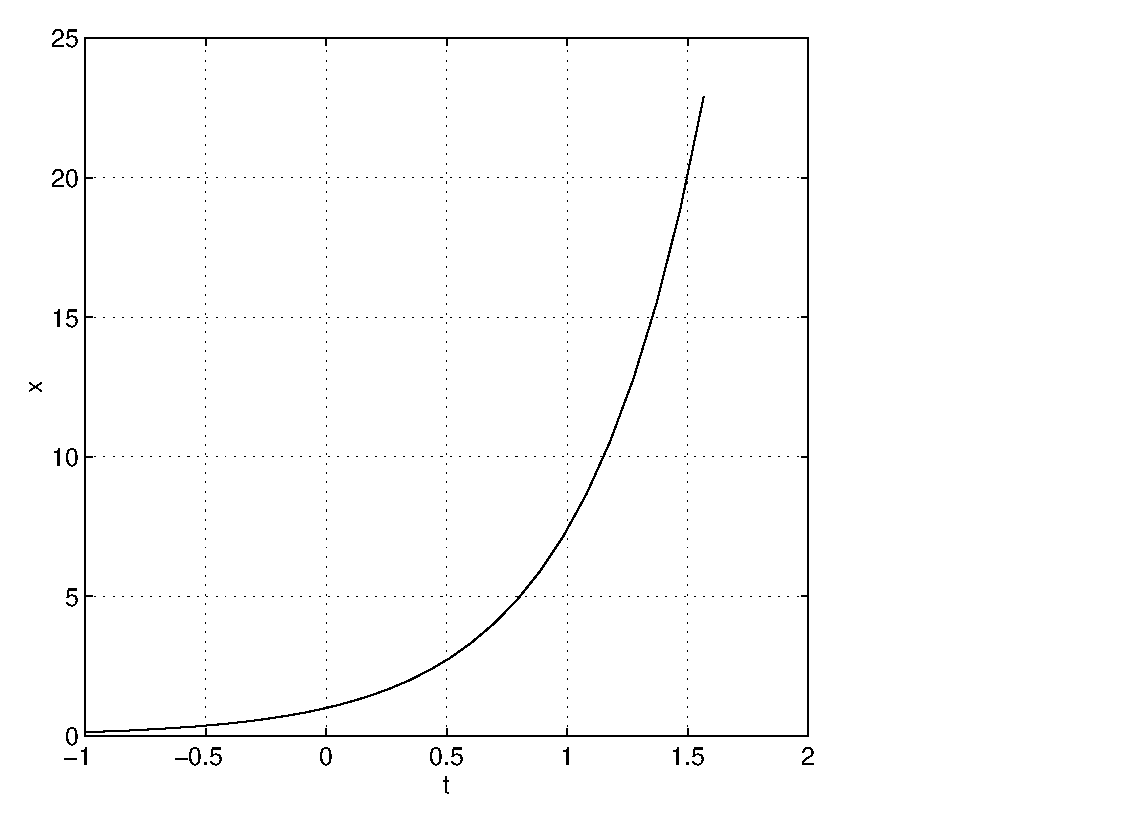
\psfig{file=../figures/plotx.eps,height=2.0in,width=3.0in}
     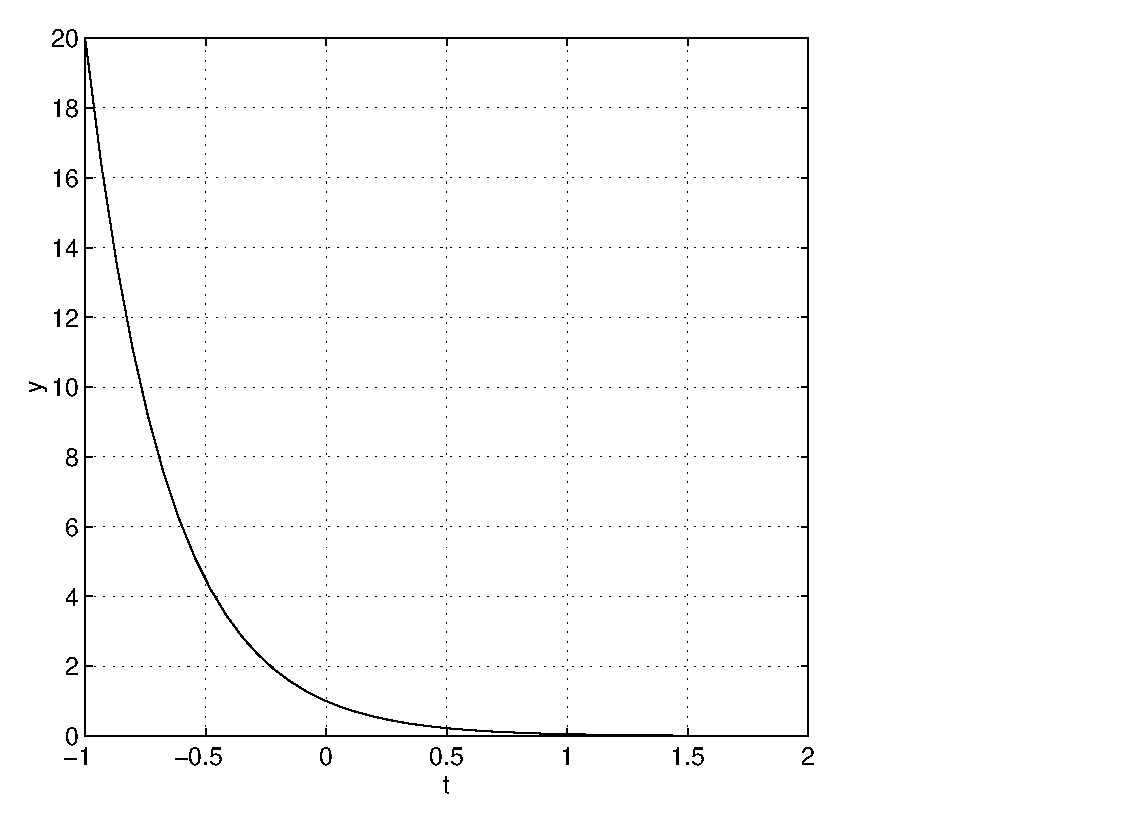
\psfig{file=../figures/ploty.eps,height=2.0in,width=3.0in}}
     \centerline{%
     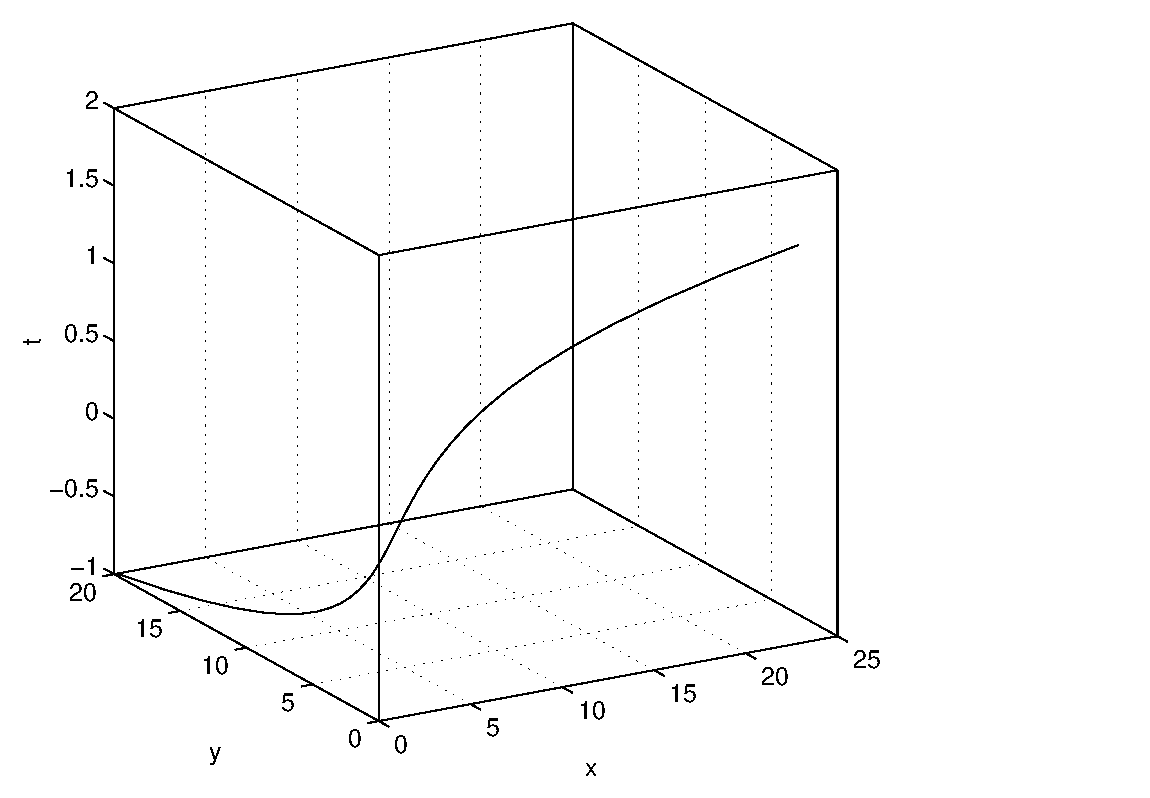
\psfig{file=../figures/plot3d.eps,width=3.0in}
     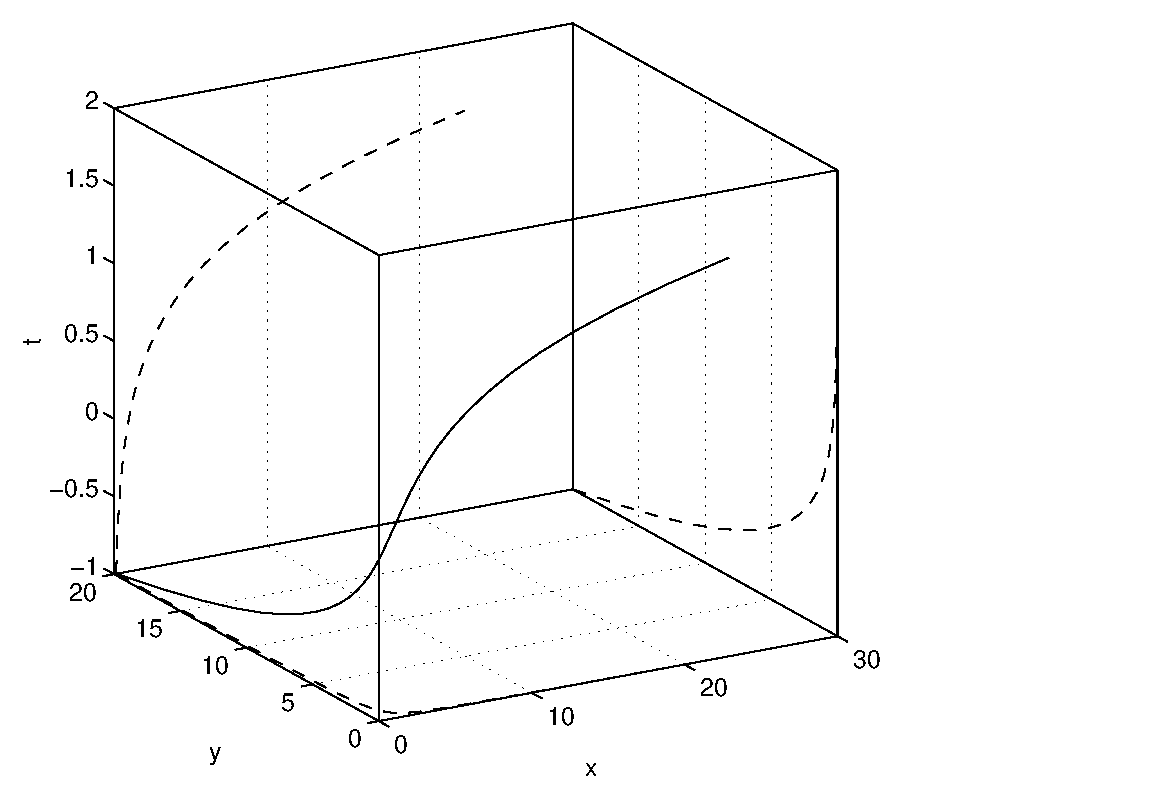
\psfig{file=../figures/plotall.eps,width=3.0in}}
     \caption{{\sf PPLANE9 Display} for \protect\eqref{lin2} with
             $a=2$, $d=-3$ and $x\in [0,25], y\in [0,20]$. The solution
             going through $(1,1)$ is shown. UL: $(t,x(t))$;
	UR: $(t,y(t))$; LL: $(x(t),y(t),t)$; LR: all plots.}
     \label{plotall}
\end{figure*}




\includeexercises



\end{document}
